%-----------------------------------------------------------------
%Author: Yan Naing Aye
%Date:   2012 Feb 24
%-----------------------------------------------------------------
\documentclass[12pt,a4paper]{report}      % Specifies the document class

\usepackage{graphicx} %for pdf, bitmapped graphics files
\usepackage{amsmath} %to facilitate writing math formulas and to improve the typographical quality
\usepackage{amssymb}  %provides an extended symbol collection
\usepackage{wasysym} %pro­vides many glyphs
\usepackage{subfigure} %for subfigures
\usepackage{epstopdf} %converts eps to pdf
%\usepackage{fullpage} %to use full page
\usepackage[table]{xcolor} %color extensions (for tables)
%\usepackage[numbers]{natbib} %reimplementation of \cite command
\usepackage{datetime} %date time
\usepackage[pdftitle={Aye-Thesis},pdfauthor={Yan Naing Aye}]{hyperref}
\hypersetup{
	colorlinks,
	citecolor=black,
	filecolor=black,
	linkcolor=black,
	urlcolor=black
}
\usepackage[font={small,sf},labelfont=bf]{caption} %to change figure caption font
%\usepackage{float} %to use figure with [H] option
%\usepackage{fancyhdr} %fancy headers
%-----------------------------------------------------------------
%Macros
\def\titleSentence{REAL-TIME HIGH PERFORMANCE DISPLACEMENT SENSING IN HANDHELD INSTRUMENT FOR MICROSURGERY}
% I use this title in several places throughout the report
% that is why I define it as \titleSentence command 
% so that I only need to change here and all will be updated accordingly
%-----------------------------------------------------------------
\newdateformat{mydate}{\THEYEAR} %year only
%\newdateformat{mydate}{\monthname[\THEMONTH] \THEYEAR} %use this for month and year
%-----------------------------------------------------------------
%\newcommand{\ip}[2]{(#1, #2)}

% Define a new command called \los to include list of symbol easily.
% It is used in ListOfSymbols.tex file
\newcommand{\los}[2]{\parbox[t]{5cm}{$#1 \dotfill$}  \parbox[t]{10cm}{#2}\\[0.6cm]}                                                    %-----------------------------------------------------------------        
\renewcommand{\bibname}{References}%change Bibliography to References                         
\renewcommand{\baselinestretch}{1.5} %linespace
%\linespread{1.6}
%-----------------------------------------------------------------
\pagestyle{headings}    %comment out usepackage{fullpage} to use headings style
%-----------------------------------------------------------------
\begin{document}        %End of preamble and beginning of text.
	%\begin{titlepage}

\begin{center}
{\LARGE  \bfseries \titleSentence}\\[1cm]

% Upper part of the page   

\includegraphics[width=10cm]{./Fig/ntu_logo.jpg}\\[1cm]    

{\Large \bfseries YAN NAING AYE}\\[2cm]

\emph{\Large Submitted in partial fulfillment of the requirements for confirmation of PhD candidature}\\[4cm]

\textsc{\large 
School of Mechanical and Aerospace Engineering\\
Division of Mechatronics and Design\\
Nanyang Technological University}\\[1cm]
\vfill

% Bottom of the page
{\large \mydate\today}

\end{center}
\end{titlepage} %Title page for comfirmation report
	\begin{titlepage}

\begin{center}

% Upper part of the page   

\includegraphics[width=10cm]{./Fig/ntu_logo.jpg}\\[3cm]  
  
{\Large  \bfseries \titleSentence}\\[1cm]
\vfill
{\Large \bfseries YAN NAING AYE}\\[1cm]
{\Large \bfseries SCHOOL OF MECHANICAL AND AEROSPACE ENGINEERING}\\[1cm]
{\Large \bfseries  2016}

\end{center}
\end{titlepage} 	%Title page for thesis hardbound
	\begin{titlepage}

\begin{center}
{\Large  \bfseries \titleSentence}\\[4cm]

{\Large \bfseries YAN NAING AYE}\\[3cm]
\vfill
\textsc{\large 
	School of Mechanical and Aerospace Engineering}\\[1cm]

{\Large \sffamily A thesis submitted to the Nanyang Technological University in partial fulfilment of the requirements for the degree of Doctor of Philosophy}\\[1cm]


% Bottom of the page
{\Large \bfseries \mydate\today}

\end{center}
\end{titlepage} 	%Title page for thesis
	%-----------------------------------------------------------------------------
	\newpage
	\pagenumbering{roman}  %added it if has Acknowledgment
	%\chapter*{Abstract}
	%\addcontentsline{toc}{chapter}{Abstract}
	\begin{abstract}
		%Overview of the system
The main focus of this research is ...

	\end{abstract}
	%-----------------------------------------------------------------
	\newpage
	\chapter*{Acknowledgments}
	\addcontentsline{toc}{chapter}{Acknowledgment}
	I would like to express my first and foremost gratitude to my thesis adviser ...
	% -----------------------------------------------------------------
	\newpage
	\addcontentsline{toc}{chapter}{Table of Contents}
	\tableofcontents
	%------------------------------------------------------------------
	\newpage
	\addcontentsline{toc}{chapter}{List of Figures}
	\listoffigures
	%-----------------------------------------------------------------
	\newpage
	\addcontentsline{toc}{chapter}{List of Tables}
	\listoftables
	\clearpage
	%-----------------------------------------------------------------
	\newpage
	\markboth{\MakeUppercase{List of Symbols and Abbreviations}}{\MakeUppercase{List of Symbols and Abbreviations}}
	\chapter*{List of Symbols and Abbreviations\hfill} 
	\addcontentsline{toc}{chapter}{List of Symbols and Abbreviations}
	%List of symbols
\los{\mathbf{A}_i=\begin{bmatrix}a_{ix} & a_{iy} & a_{iz}\end{bmatrix}^T}{Vector representing acceleration at location \{i\}}
\los{\text{BMFLC}}{Band-limited multiple Fourier linear combiner}

	\clearpage
	%-----------------------------------------------------------------
	\newpage
	\pagenumbering{arabic}
	\setcounter{page}{1}
%-----------------------------------------------------------------
\chapter{Introduction}
\label{ch:Introduction}

%------------------------------------------------------------------------------
\section{Background}

Physiological tremor is the most common involuntary motion affecting micromanipulation \cite{Aye1209:Vision}. 

\section{Organization}

Chapter \ref{ch:Introduction} defines the problem and objectives of this report. 

%-----------------------------------------------------------------
\chapter{Literature Review}
\label{ch:Literature}
%------------------------------------------------------------------------------


%-----------------------------------------------------------------
\chapter{Design of the Sensing System}
\label{ch:System}
%------------------------------------------------------------------------------

\section{System Overview}
\label{Sec:SystemOverview}

The \textit{ITrem2} sensing system consists of two sub-systems, the inertial measurement system and the vision system. 

\begin{figure*}[htbp!]
 \centering
 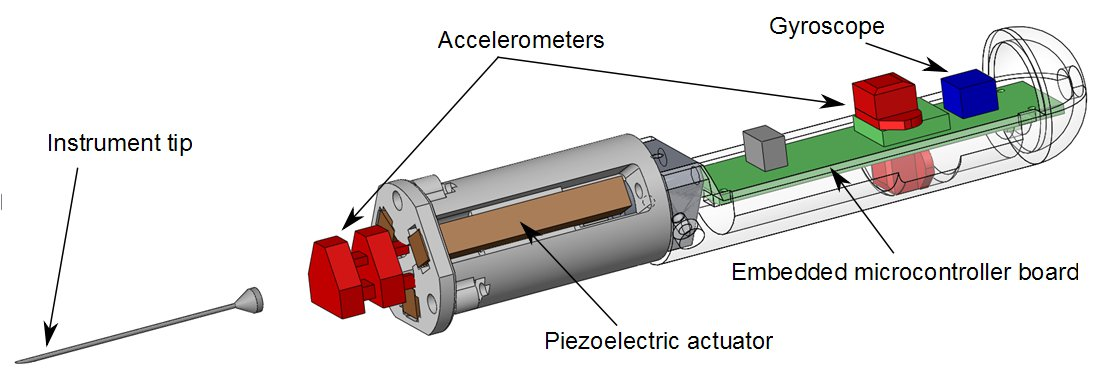
\includegraphics[width=1\textwidth]{./Fig/Fig_InstrumentComponents.jpg}
 \caption{\textit{ITrem2} schematic}
 \label{Fig_InstrumentComponents}
\end{figure*}

%-----------------------------------------------------------------
\chapter{Conclusion}
\label{ch:Conclusion}


%-----------------------------------------------------------------
\appendix
\chapter{Error Calculation}
%------------------------------------------------------------------------------
\section{Error Between Two Sinusoidal Signals}
\label{Ap_Err2S}

The motion equation of an assumed sinusoidal tremor with amplitude, $X_1$, and angular frequency, $\omega$, is represented by
\begin{equation}
x_1(t)= X_1 \cos \omega t.
\end{equation}

%-----------------------------------------------------------------
\bibliographystyle{ieeetr}
%\bibliographystyle{cell}
%\bibliographystyle{apalike}
\bibliography{./Files/Ref}
\addcontentsline{toc}{chapter}{References}
% -----------------------------------------------------------------
\end{document}
% -----------------------------------------------------------------